\documentclass[11pt,a4paper]{article}
\usepackage[spanish,es-nodecimaldot]{babel}
\usepackage[margin=2.05cm]{geometry}
\usepackage{amsmath,amssymb,graphicx,booktabs,tabularx,array,xcolor,enumitem}
\usepackage[unicode,colorlinks=true,linkcolor=teal,urlcolor=teal]{hyperref}
\hypersetup{pdftitle={Spin Network Laboratory: descripción completa del Workshop 1},pdfauthor={Dairon Steven Cabascango Erazo},pdfsubject={Avance funcional: estructuras de datos, grafo, física e interfaz SFML}}
\setlength{\parindent}{0pt}
\setlength{\emergencystretch}{2em}
\setlength{\parskip}{0.48em}
\setlist[itemize]{topsep=3pt,itemsep=2pt,leftmargin=1.5em}
\setlist[enumerate]{topsep=3pt,itemsep=2pt,leftmargin=1.8em}
\renewcommand{\arraystretch}{1.16}
\newcolumntype{Y}{>{\raggedright\arraybackslash}X}
\newcommand{\archivo}[1]{\texttt{\detokenize{#1}}}
\newcommand{\fuente}[1]{\par\vfill{\footnotesize\color{gray}Base de implementación: #1.}}
\begin{document}
\begin{center}
{\small\scshape Documento de descripción del proyecto}\par
\vspace{1.2cm}
{\Huge\bfseries Spin Network Laboratory}\par
\vspace{0.45cm}
{\Large Simulador dinámico de redes topológicas\par en C++17 y SFML}\par
\vspace{0.8cm}
{\large\bfseries Workshop 1: avance funcional}\par
\vspace{0.8cm}
\end{center}
\textbf{Integrantes del equipo}\par
Dairon Steven Cabascango Erazo.

\textbf{Descripción del proyecto}\par
Spin Network Laboratory es un sistema computacional inspirado en redes de espín que permite construir, visualizar, modificar y explorar grafos dinámicos. El avance combina estructuras de datos personalizadas, administración explícita de memoria, interacción gráfica e integración numérica. Los vértices se almacenan en una tabla hash propia y sus conexiones se representan mediante listas simplemente enlazadas. Una interfaz SFML presenta la red y permite editarla mientras un modelo artificial de fuerzas organiza su geometría.

\textbf{Componentes implementados actualmente en esta entrega}\par
Lista simplemente enlazada; tabla hash FNV-1a con encadenamiento y rehash; grafo simple no dirigido; modelo de vértices y aristas; motor de fuerzas; integrador Velocity Verlet con paso fijo; controlador de interacción; renderizado y panel básico SFML; consola auxiliar; pruebas automatizadas y demo web independiente.

\textbf{Enlace al repositorio de GitHub}\par
\url{https://github.com/stevencabascango/Spin-Newtwork-of-Quantum-Gravity.git}

\textbf{Alcance del documento}\par
Se describe exclusivamente la versión conservada en la carpeta \archivo{Workshop 1}. La implementación de la segunda entrega se mantiene separada. Las fuerzas son herramientas de visualización: el programa no constituye una simulación completa de gravedad cuántica ni una implementación de la dinámica de redes de espín de LQG.

\vfill
{\small Descripción preparada a partir del código local y de sus pruebas. Estado de comprobación: 10 de octubre de 2026.}
\newpage

\section{Descripción completa, propósito y objetivos}
\subsection{Problema que aborda el proyecto}
Un grafo representa entidades y relaciones entre ellas. Cuando sus vértices o conexiones se modifican, la estructura debe conservar referencias válidas, conteos correctos y una representación coherente. Además, un dibujo estático resulta insuficiente para observar cómo cambia la geometría al conectar, mover o eliminar elementos.

El proyecto integra ambas necesidades: construye un núcleo de almacenamiento y edición con estructuras propias y lo conecta con un simulador visual. La geometría evoluciona mediante fuerzas artificiales, mientras la topología cambia únicamente por las operaciones explícitas del usuario. Mover un nodo modifica su posición, pero no crea ni elimina conexiones.

\subsection{Objetivo general}
Desarrollar un avance ejecutable en C++17 capaz de almacenar, editar y visualizar un grafo no dirigido, utilizando una tabla hash y listas enlazadas propias, y actualizar sus posiciones mediante integración numérica de paso fijo.

\subsection{Objetivos específicos}
\begin{enumerate}
\item Implementar una lista simple con inserción, búsqueda, eliminación, limpieza e iteración.
\item Implementar una tabla hash con FNV-1a, colisiones por encadenamiento y redimensionamiento controlado.
\item Representar vértices por identificadores y conexiones recíprocas sin punteros colgantes entre vértices.
\item Mantener las reglas de grafo simple: sin lazos, sin aristas duplicadas y sin extremos inexistentes.
\item Incorporar atracción elástica, repulsión regularizada y amortiguamiento.
\item Separar el paso físico del ritmo de renderizado mediante Velocity Verlet y un acumulador temporal.
\item Permitir selección, arrastre, fijación, creación, conexión, eliminación y pausa en SFML.
\item Comprobar estructuras, dinámica e interacción con pruebas reproducibles.
\end{enumerate}

\subsection{Interpretación del modelo}
El término \archivo{QuantumVertex} pertenece al lenguaje conceptual del proyecto: computacionalmente es un vértice etiquetado con estado físico artificial. El espín de una arista es una etiqueta semientera positiva. No se imponen reglas de acoplamiento SU(2), amplitudes cuánticas, restricciones gravitacionales ni una correspondencia con la dinámica física de la gravedad cuántica.

La contribución de esta entrega es computacional y académica: mostrar que estructuras personalizadas pueden sostener un grafo editable y una visualización dinámica. La validación de ese software es distinta de demostrar una teoría física.
\fuente{\archivo{README.md}, \archivo{QuantumGraph.hpp} y \archivo{SimulationController.hpp}}
\newpage

\section{Arquitectura, objetos y administración de memoria}
\subsection{Organización por responsabilidades}
\begin{verbatim}
DesktopApplication -> InputController / GraphRenderer / HUD
        |
        +-- SimulationController
               +-- QuantumGraph
               |      +-- HashTable<uint64_t, QuantumVertex>
               |                    +-- QuantumVertex
               |                          +-- SinglyLinkedList<SpinEdge>
               +-- ForceEngine / VerletIntegrator / FixedStepClock
\end{verbatim}
El núcleo y la lógica de interacción no necesitan abrir una ventana para ejecutarse en las pruebas. SFML se utiliza en la capa de presentación: ventana, eventos, dibujo y texto. Esta separación permite evaluar fallos de estructuras o física independientemente del sistema gráfico.

\subsection{Vértices y aristas}
\begin{tabularx}{\linewidth}{@{}p{3.55cm}Y@{}}\toprule
Objeto & Información almacenada \\\midrule
\archivo{QuantumVertex} & ID; masa y volumen; posición actual y anterior; velocidad, aceleración y fuerza; estado \archivo{pinned}; lista simple de conexiones. \\
\archivo{SpinEdge} & ID lógico de arista, \archivo{targetId}, espín, longitud natural y rigidez. \\
\archivo{Vec2} & Dos componentes reales y operaciones vectoriales elementales. \\
\archivo{PhysicsParameters} & Rigidez global, repulsión, amortiguamiento, regularización y paso físico fijo. \\\bottomrule
\end{tabularx}
El volumen se conserva como atributo del vértice; no se utiliza para calcular las fuerzas de esta versión. La dinámica usa masa, posiciones, velocidades y parámetros de las conexiones. Esto evita atribuir a un campo almacenado una función que todavía no tiene.

\subsection{Propiedad de los recursos}
La tabla posee los vértices. Cada vértice posee su lista de adyacencias. Los nodos de hash y lista poseen el nodo siguiente mediante \archivo{std::unique_ptr}; el puntero de cola es observador. No se usan \archivo{new} y \archivo{delete} manuales para administrar esos nodos.

Las aristas contienen IDs de destino y no punteros directos al otro vértice. Por ello, un rehash puede reconstruir el almacenamiento sin alterar el significado de las conexiones. Los punteros devueltos por \archivo{findVertex} son observadores temporales y no deben conservarse tras rehash, eliminación o asignación.

\subsection{Copia, movimiento y limpieza}
Las listas y tablas admiten copia profunda: copiar un grafo duplica sus vértices y listas internas. El movimiento permite transferir estructuras y reutilizar el origen. La destrucción de las cadenas es iterativa para evitar una recursión proporcional al número de nodos. Estas capacidades preparan el historial de la segunda entrega, pero no significan que el historial C++ esté incluido en Workshop 1.
\fuente{\archivo{include/Core/}, \archivo{include/DataStructures/} y \archivo{src/Graphics/}}
\newpage

\section{Lista simplemente enlazada personalizada}
\subsection{Estructura interna}
\archivo{SinglyLinkedList<T>} contiene una cabeza propietaria, una cola observadora y un contador. Cada nodo almacena un valor de tipo \archivo{T} y un \archivo{unique_ptr} al siguiente. La lista se usa para las adyacencias de cada vértice, por lo que el costo de recorrerla depende de su grado.
\begin{verbatim}
head -> [valor | next] -> [valor | next] -> [valor | null]
                                                   ^
                                              tail (observador)
\end{verbatim}

\subsection{Operaciones implementadas}
\begin{tabularx}{\linewidth}{@{}p{4cm}Yp{1.8cm}@{}}\toprule
Operación & Comportamiento & Costo \\\midrule
\archivo{pushFront} & Inserta al inicio; establece cola cuando estaba vacía. & $O(1)$ \\
\archivo{pushBack} & Inserta al final sin recorrer toda la cadena. & $O(1)$ \\
\archivo{find}, \archivo{contains} & Buscan por igualdad; la búsqueda admite acceso constante o mutable. & $O(n)$ \\
\archivo{remove} & Elimina la primera coincidencia por valor. & $O(n)$ \\
\archivo{removeIf} & Elimina por predicado; útil para buscar una arista por destino. & $O(n)$ \\
\archivo{clear} & Desmonta la cadena y deja cabeza/cola vacías. & $O(n)$ \\
\archivo{size}, \archivo{empty} & Consultan el contador y el estado vacío. & $O(1)$ \\
\archivo{begin}, \archivo{end} & Permiten iteración sin exponer los nodos propietarios. & Inicio $O(1)$ \\\bottomrule
\end{tabularx}

\subsection{Eliminación correcta de cabeza y cola}
La eliminación opera sobre el enlace propietario que apunta al nodo encontrado. Ese enlace puede ser la cabeza o el \archivo{next} del nodo anterior. El siguiente nodo ocupa el enlace del retirado. Si se elimina la cola, el observador pasa al anterior; si era el único elemento, queda nulo. El contador se reduce una vez por eliminación efectiva.

\subsection{Copias independientes y pruebas}
La copia reconstruye una nueva cadena con los valores del origen, evitando compartir nodos internos. La asignación usa un temporal e intercambio. El movimiento deja el origen vacío y permite insertar nuevos valores en él.

Las pruebas comprueban inserción por ambos extremos, búsquedas existentes y ausentes, eliminación de cabeza y cola, reinserción después de vaciar, iteración constante y copia/movimiento. Se construye también una lista de 10\,000 elementos para comprobar que una copia permanece independiente y que la limpieza funciona sin recurrir a liberaciones manuales.
\fuente{\archivo{SinglyLinkedList.hpp} y \archivo{tests/test_core.cpp}}
\newpage

\section{Tabla hash: FNV-1a, colisiones y rehash}
\subsection{Almacenamiento por identificador}
\archivo{HashTable<uint64_t, QuantumVertex>} relaciona el ID con el vértice. Un arreglo de buckets inicia cadenas propias de nodos clave--valor. Una búsqueda calcula el bucket y recorre su cadena; no utiliza \archivo{std::unordered_map} como sustituto de la tabla evaluada.

\subsection{Función hash implementada}
Para bytes $b_i$ de la clave, FNV-1a de 64 bits se calcula como
\[
h_0=14695981039346656037,\qquad
h_{i+1}=(h_i\mathbin{\mathrm{XOR}}b_i)\,1099511628211\pmod{2^{64}}.
\]
El índice es $h(k)\bmod m$, donde $m$ es el número de buckets. Las claves enteras se codifican en bytes little-endian para obtener un resultado independiente del orden de bytes del procesador. La tabla también admite cadenas y un hash alternativo inyectable para las pruebas.

\subsection{Resolución de colisiones}
Dos claves con el mismo índice se guardan en la misma cadena, pero siguen distinguiéndose por su valor de clave. Insertar un ID repetido devuelve rechazo y no sobrescribe silenciosamente el vértice. Eliminar una entrada repara el enlace de la cadena.
\begin{verbatim}
bucket[0] -> [clave A, valor] -> [clave B, valor] -> null
bucket[1] -> null
bucket[2] -> [clave C, valor] -> null
\end{verbatim}

\subsection{Factor de carga y redimensionamiento}
El factor de carga es $\alpha=n/m$. Antes de una inserción que supere $0.75$, la tabla solicita una capacidad mayor. El rehash reconstruye una tabla temporal y la intercambia con el original únicamente después de completar las inserciones. Copiar valores durante ese proceso incluye copiar las adyacencias del vértice.

La capacidad finalmente elegida puede superar una solicitud demasiado pequeña para respetar el factor de carga. Los observadores de vértices pueden invalidarse: el código no debe depender de conservar sus direcciones durante un rehash.

\subsection{API, costos y evidencia}
La API incluye \archivo{insert}, \archivo{remove}, \archivo{find}, \archivo{contains}, \archivo{clear}, \archivo{size}, \archivo{capacity}, \archivo{loadFactor} y \archivo{rehash}. El costo esperado de consulta es $O(1)$ con distribución adecuada; con colisiones patológicas puede llegar a $O(n)$.

Las pruebas insertan y buscan 5\,000 vértices, rechazan duplicados, reconstruyen a 16\,384 buckets y eliminan todas las entradas. Un hash constante fuerza 1\,000 claves al mismo bucket y verifica consultas y eliminaciones. También se comprueba FNV-1a de \archivo{hello} contra el valor esperado \archivo{0xa430d84680aabd0b}.
\fuente{\archivo{HashTable.hpp} y \archivo{tests/test_core.cpp}}
\newpage

\section{Grafo no dirigido y componentes del núcleo}
\subsection{Representación y contratos}
El grafo es $G=(V,E)$, simple y no dirigido. Los vértices están indexados en la hash y cada uno posee su lista de adyacencias. Crear una conexión entre $a$ y $b$ inserta los registros $a\to b$ y $b\to a$ con el mismo ID lógico. El contador de aristas aumenta una vez, no dos.

Se rechazan lazos ($a=b$), duplicados y extremos inexistentes. Masa no positiva, posiciones no finitas y parámetros de arista inválidos producen rechazo o excepción según la operación. El espín debe ser positivo y semientero; la longitud natural, positiva; la rigidez, no negativa.

\subsection{Operaciones implementadas}
\begin{tabularx}{\linewidth}{@{}p{4.9cm}Y@{}}\toprule
Operación & Función \\\midrule
\archivo{addVertex}, \archivo{removeVertex} & Crear o eliminar vértices e incidentes. \\
\archivo{addEdge}, \archivo{removeEdge} & Mantener las dos adyacencias y el conteo lógico. \\
\archivo{findVertex}, \archivo{containsVertex} & Localizar vértices por ID. \\
\archivo{vertexCount}, \archivo{numberOfEdges} & Consultar tamaños del grafo. \\
\archivo{degree}, \archivo{neighbors} & Consultar conexiones de un vértice. \\
\archivo{ids}, \archivo{forEachVertex} & Recorrer y obtener IDs ordenados. \\
\archivo{clear}, \archivo{rehash} & Limpiar o reorganizar almacenamiento. \\\bottomrule
\end{tabularx}
Se conservan también nombres cortos de la API original: \archivo{size}, \archivo{edgeCount} y \archivo{contains}. El código externo no debe modificar directamente las adyacencias: las operaciones del grafo mantienen su reciprocidad.

\subsection{Eliminación y consistencia}
Para eliminar un vértice se obtienen primero sus vecinos. Se retira cada arista en ambos extremos, se reduce el contador y finalmente se elimina el vértice de la hash. Así ningún vecino conserva una conexión al ID eliminado. Si falla la creación de la segunda adyacencia de una arista, se retira la primera antes de propagar el error.

\subsection{Métricas complementarias ya disponibles}
El núcleo conserva funciones básicas de análisis y una consola: número de vértices/aristas, grado, componentes conexas y ciclos independientes. Si $C$ es el número de componentes conexas, para un grafo 1D se usan $\beta_0=C$, $\beta_1=E-V+C$ y $\chi=V-E$. Estas funciones son un complemento del avance; no equivalen al panel analítico, lista doble e historial C++ de la segunda entrega.

\subsection{Prueba representativa}
Un grafo de 1\,000 vértices y 5\,000 aristas tiene grado 10 en cada nodo del caso probado. Al eliminar el vértice 0 se retiran sus 10 conexiones y el conteo baja a 4\,990. Su copia mantiene el grafo original; reinsertar el ID eliminado crea un vértice aislado.
\fuente{\archivo{QuantumGraph.hpp}, \archivo{GraphMetrics.hpp} y \archivo{tests/test_core.cpp}}
\newpage

\section{Dinámica artificial y parámetros}
\subsection{Modelo de visualización}
Las fuerzas buscan una distribución visual comprensible: resortes para las conexiones, repulsión entre pares y amortiguamiento para reducir oscilaciones. No modifican las conexiones. Las coordenadas y parámetros utilizan unidades internas de simulación; no se presentan como mediciones físicas en unidades SI.

Para posiciones $\mathbf{x}_i$, se define $\boldsymbol\Delta_{ij}=\mathbf{x}_j-\mathbf{x}_i$ y $r_{ij}=\|\boldsymbol\Delta_{ij}\|$. La fuerza del resorte implementada sobre $i$ es
\[
\mathbf{F}^{s}_{ij}=k_{\mathrm{global}}k_{ij}(r_{ij}-L_{ij})
\frac{\boldsymbol\Delta_{ij}}{r_{ij}+\varepsilon_s}.
\]
Cuando $r_{ij}>L_{ij}$ atrae hacia $j$; cuando es menor, separa. Cada arista lógica se evalúa una vez y contribuye con signos opuestos a sus extremos.

\subsection{Repulsión regularizada}
Para un par distinto,
\[
\mathbf{F}^{r}_{ij}=-\frac{k_r}{r_{ij}^2+\varepsilon^2}\widehat{\boldsymbol\Delta}_{ij}.
\]
La regularización usa $\varepsilon=5$ en el valor inicial. Si dos nodos coinciden, se elige una dirección determinista basada en los IDs; esto produce separación sin dividir por cero. La interacción se evalúa para todos los pares, de costo $O(V^2)$. El espín es una etiqueta: no modifica directamente las fuerzas de este avance.

\subsection{Amortiguamiento y masa}
Se utiliza $\mathbf{F}^{d}_i=-\gamma\mathbf{v}_i$ y $\mathbf{a}_i=\mathbf{F}_i/m_i$. Las fuerzas conservativas se acumulan en \archivo{ForceEngine}; el amortiguamiento se aplica por separado en el integrador mediante una exponencial que incluye la masa. Un nodo fijo no recibe masa infinita: \archivo{pinned=true} impide avanzar su posición y mantiene velocidad cero.

\begin{tabularx}{\linewidth}{@{}Yp{3cm}Y@{}}\toprule
Parámetro inicial & Valor & Papel \\\midrule
Rigidez global & $2.0$ & Escala los resortes de aristas. \\
Repulsión & $12\,000$ & Evita agrupación excesiva. \\
Amortiguamiento & $2.0$ & Reduce velocidades y oscilaciones. \\
Regularización & $5.0$ & Acota repulsión a distancias pequeñas. \\
Longitud de los presets & $90$ & Longitud natural por arista. \\
Masa de presets & $1.0$ & Respuesta inercial artificial. \\\bottomrule
\end{tabularx}
Para una interpretación dimensional interna, rigidez efectiva tiene dimensión $M/T^2$, repulsión $ML^3/T^2$ y amortiguamiento $M/T$. Los números son parámetros del modelo gráfico, no constantes gravitacionales.
\fuente{\archivo{ForceEngine.hpp}, \archivo{PhysicsParameters.hpp} y \archivo{QuantumVertex.hpp}}
\newpage

\section{Velocity Verlet y actualización de paso fijo}
\subsection{Algoritmo conservativo}
Velocity Verlet divide el impulso de velocidad en dos medios pasos. Primero se calculan fuerzas en la posición actual; luego se avanza la posición y se recalculan fuerzas:
\begin{align*}
\mathbf{v}_{n+1/2}&=\mathbf{v}_n+\tfrac{\Delta t}{2}\mathbf{a}_n,\\
\mathbf{x}_{n+1}&=\mathbf{x}_n+\Delta t\,\mathbf{v}_{n+1/2},\\
\mathbf{a}_{n+1}&=\mathbf{F}(\mathbf{x}_{n+1})/m,\\
\mathbf{v}_{n+1}&=\mathbf{v}_{n+1/2}+\tfrac{\Delta t}{2}\mathbf{a}_{n+1}.
\end{align*}
La versión implementada incorpora amortiguamiento con separación simétrica de operadores. Para $d=\exp[-\gamma\Delta t/(2m)]$, realiza
\[
\mathbf{v}_{1/2}=d\mathbf{v}_n+\tfrac{\Delta t}{2}\mathbf{a}_n,
\qquad
\mathbf{v}_{n+1}=d\bigl(\mathbf{v}_{1/2}+\tfrac{\Delta t}{2}\mathbf{a}_{n+1}\bigr).
\]
La posición se avanza con $\mathbf{v}_{1/2}$. Esto evita tratar el amortiguamiento dependiente de velocidad como una fuerza dependiente únicamente de posición.

\subsection{Reloj físico independiente de FPS}
El paso fijo es $\Delta t=1/120$ s. \archivo{FixedStepClock} acumula el tiempo transcurrido entre frames y ejecuta pasos completos. A 60 FPS, normalmente se realizan dos pasos físicos por frame; no se utiliza directamente el tiempo variable del frame como paso de integración.

Pausar reinicia el acumulador para no recuperar el tiempo de pausa. Una suspensión larga se limita a $0.1$ s de recuperación, como máximo 12 pasos. Esa política descarta tiempo deliberadamente tras bloqueos prolongados; la equivalencia entre FPS se comprueba en condiciones sin esos bloqueos.

\subsection{Fijación, arrastre y comprobaciones}
Un vértice fijo o arrastrado mantiene su posición durante la física y tiene velocidad cero. El arrastre conserva el desplazamiento entre el centro del nodo y el punto donde se agarró, evitando un salto inicial. La posición anterior y aceleración se actualizan como parte del estado numérico.

Las pruebas comparan el resultado tras un segundo a 30, 60 y 144 FPS con tolerancia $10^{-8}$ en posiciones. Un oscilador sin amortiguamiento mantiene error relativo de energía inferior a $0.1\%$ tras 1\,200 pasos; la prueba amortiguada confirma disipación. Una masa libre cumple el decaimiento esperado $v(t)=v(0)e^{-\gamma t/m}$. Estas son comprobaciones de los casos ejecutados, no una garantía universal de estabilidad para cualquier parámetro o grafo.
\fuente{\archivo{VerletIntegrator.hpp} y \archivo{tests/test_physics.cpp}}
\newpage

\section{Interfaz SFML, controles y demo complementaria}
\subsection{Presentación implementada}
\archivo{GraphRenderer} dibuja aristas como segmentos, vértices como círculos e IDs junto a los nodos. \archivo{HUD} presenta herramientas, conteos, estado de pausa, parámetros y FPS. \archivo{InputController} traduce eventos y coordenadas de pantalla a acciones sobre el grafo; la cámara permite encuadrar sin alterar la geometría.

\begin{tabularx}{\linewidth}{@{}Yp{6.9cm}@{}}\toprule
Acción & Control del Workshop 1 \\\midrule
Seleccionar / arrastrar & Mouse izquierdo; herramienta Seleccionar o \archivo{S}. \\
Agregar vértice & Botón Agregar y clic; \archivo{A} en el lienzo. \\
Crear arista & \archivo{C} o herramienta Conectar; origen y destino. \\
Eliminar seleccionado / bajo puntero & \archivo{Delete} / \archivo{D} y clic. \\
Pausa / fijación / posiciones & \archivo{Space} / \archivo{P} / \archivo{R}. \\
Repulsión / rigidez / amortiguamiento & Flechas arriba/abajo; corchetes; coma/punto. \\
Red inicial / red de 100 nodos & \archivo{1} / \archivo{2}. \\
Encuadrar / cerrar & \archivo{F} / \archivo{Esc}. \\\bottomrule
\end{tabularx}
La red inicial tiene 20 nodos y 43 aristas; la configuración de 100 nodos tiene 261 aristas. El límite de interacción visual es 500 vértices, independiente de la capacidad de la tabla hash. Reiniciar posiciones conserva topología y fijaciones.

\subsection{Demo web independiente}
\begin{center}
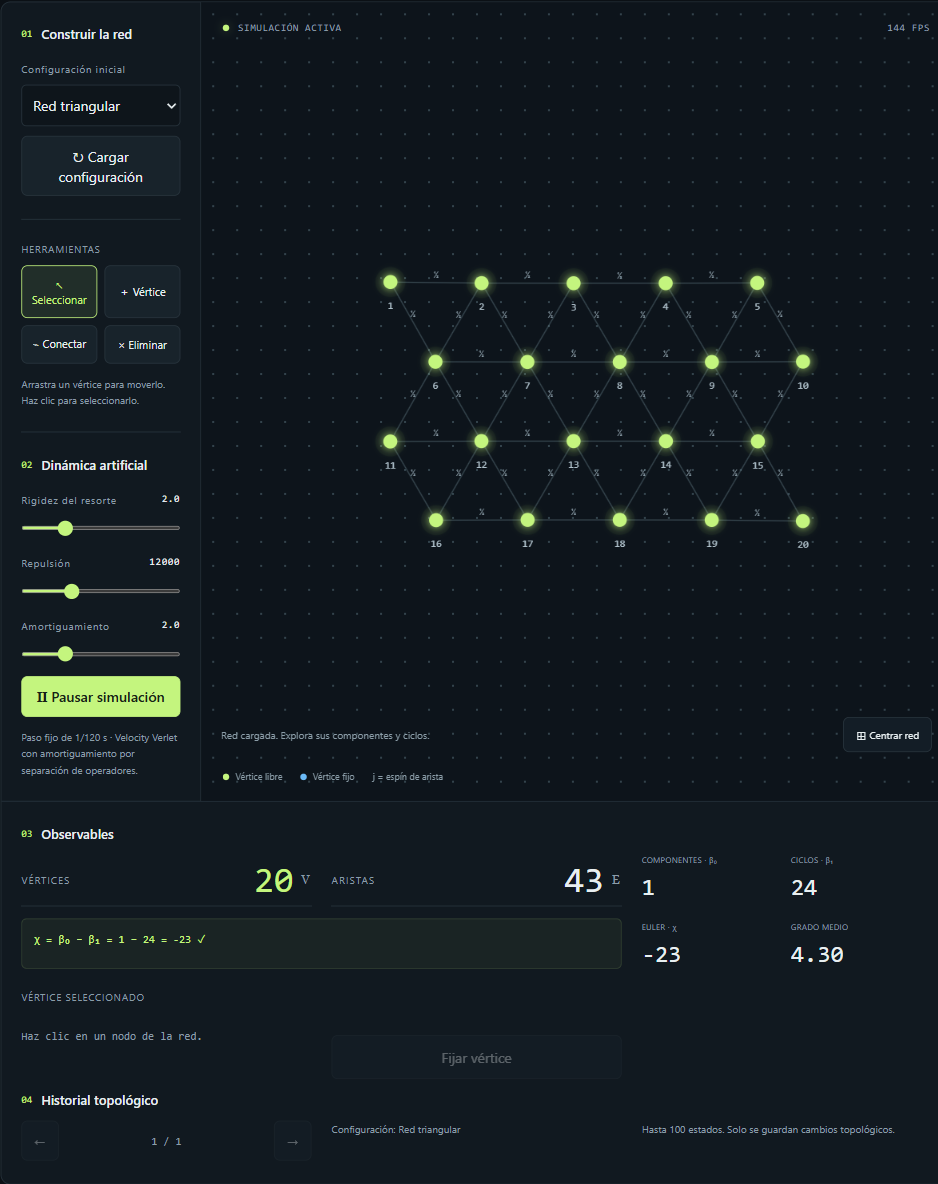
\includegraphics[width=0.86\linewidth,height=6.1cm,keepaspectratio]{../screenshots/workshop1-web.png}\\[-1mm]
{\footnotesize Captura real de la demo web del avance en Brave; no es una captura SFML.}
\end{center}
La página \archivo{site/dist/index.html} es un programa JavaScript independiente y puede abrirse sin servidor. Muestra edición, fuerzas y métricas; su historial web es complementario y no acredita una lista doble o historial C++ del Workshop 1. Sus cambios se pierden al recargar.

La aplicación nativa está implementada y compilada, pero la pantalla X11 fue bloqueada en el entorno restringido. Por tanto, el documento distingue controles probados en el controlador de una validación visual completa de la ventana SFML, que sigue pendiente.
\fuente{\archivo{src/Graphics/}, \archivo{SimulationController.hpp} y captura local de la demo web}
\newpage

\section{Pruebas, resultados y complejidades}
\subsection{Evidencia del avance}
El Workshop 1 tiene tres suites: \archivo{test_core}, \archivo{test_physics} y \archivo{test_interaction}. Sus binarios se ejecutaron nuevamente el 10 de octubre de 2026 y finalizaron correctamente. Los resultados se respaldan en las aserciones de sus fuentes; no se sustituyen por una inspección visual del código.

\begin{tabularx}{\linewidth}{@{}p{3.6cm}Y@{}}\toprule
Caso comprobado & Resultado \\\midrule
Hash propia & Inserción/búsqueda de 5\,000 vértices; duplicados rechazados; rehash y eliminación completa. \\
Colisiones & 1\,000 claves forzadas a un bucket; búsqueda y borrado de extremos/interior. \\
Lista simple & Operaciones, copia/movimiento y cadena de 10\,000 elementos. \\
Grafo & 1\,000 vértices, 5\,000 aristas y retiro de conexiones incidentes. \\
Estabilidad numérica & 100 nodos y 261 aristas durante 7\,200 pasos: 60 s simulados, estados finitos. \\
Independencia de FPS & Estados coincidentes en el caso probado a 30/60/144 FPS. \\
Interacción & Creación, conexión, rechazo de lazos/duplicados, arrastre, fijación, pausa y eliminación. \\\bottomrule
\end{tabularx}

\subsection{Costos de los algoritmos}
\begin{tabularx}{\linewidth}{@{}Yp{6.8cm}@{}}\toprule
Operación & Costo / alcance \\\midrule
Lista: insertar al frente/final & $O(1)$. Búsqueda/eliminación: $O(n)$. \\
Hash: consulta & $O(1)$ esperado; $O(V)$ en cadenas patológicas. \\
Rehash / copia de grafo & $O(V+E)$ esperado; colisiones patológicas pueden encarecer reconstrucción. \\
Fuerzas / paso Verlet & $O(V^2+E)$ esperado; dos evaluaciones de fuerzas. \\
Dibujo & $O(V+E)$ esperado. \\
IDs ordenados & $O(V\log V)$; auxiliar para reinicio y recorridos. \\\bottomrule
\end{tabularx}
Estos costos suponen cadenas hash razonablemente distribuidas. Copiar un vértice incluye sus adyacencias. La estabilidad de 100 nodos no autoriza prometer rendimiento para millones de elementos.

\subsection{Comprobaciones pendientes}
Los registros del avance indican ASan/UBSan satisfactorios con \archivo{detect_leaks=0}. LeakSanitizer no funcionó bajo ptrace: no se afirma ausencia de fugas verificada. Tampoco se comprobó la ventana SFML en el sandbox ni la compilación Windows/Code::Blocks. La prueba \archivo{--smoke-test} y el guion manual están preparados para un escritorio habilitado.
\fuente{\archivo{tests/test_core.cpp}, \archivo{test_physics.cpp}, \archivo{test_interaction.cpp} y \archivo{docs/validation.md}}
\newpage

\section{Archivos, ejecución y enlace al repositorio}
\subsection{Entrega del Workshop 1}
\begin{verbatim}
Workshop 1/
  main.cpp                  SpinNetworkLaboratory.cbp
  CMakeLists.txt            README.md / ENTREGA.txt
  include/                  src/
  tests/                    assets/fonts/
  docs/architecture.md      docs/validation.md
  docs/report/              site/dist/
  tools/                    bin/ / .deps/sfml/
\end{verbatim}
La carpeta conserva el avance de manera independiente. Los fuentes, recursos, configuración de compilación y pruebas están incluidos. El SDK local y binarios suministrados son para Linux x86\_64; no son ejecutables de Windows.

\subsection{Compilación y ejecución reproducibles}
Desde la carpeta del Workshop 1, con GCC C++17 y SFML 2.6 compatibles:
\begin{verbatim}
./tools/build.sh
./bin/spin_network
./tools/build.sh --core-only
./bin/spin_network --smoke-test
\end{verbatim}
El modo \archivo{--core-only} prueba estructuras, física e interacción sin SFML. Con CMake se usan \archivo{cmake -S . -B build}, \archivo{cmake --build build} y \archivo{ctest --test-dir build --output-on-failure}. Si se utiliza el SDK local, debe indicarse su prefijo en la configuración.

En Windows se abre \archivo{SpinNetworkLaboratory.cbp} en Code::Blocks, se configura un SDK SFML 2.6 para MinGW compatible con el compilador, se enlazan graphics/window/system y se colocan las DLL y recursos junto al programa. Las instrucciones de integración se apoyan en la documentación oficial de SFML \cite{sfml}.

\subsection{Repositorio proporcionado}
\url{https://github.com/stevencabascango/Spin-Newtwork-of-Quantum-Gravity.git}

El enlace se reproduce exactamente como fue facilitado por el integrante. El contenido descrito y las pruebas corresponden a la copia local del Workshop 1; este documento no certifica que el estado remoto sea idéntico. La segunda entrega agrupa lista doble, historial C++, undo/redo, panel analítico final y refinamiento; esas funcionalidades no se atribuyen al avance descrito aquí.

\subsection{Referencias y preparación del documento}
{\footnotesize
\begin{thebibliography}{9}
\bibitem{sfml} SFML. \emph{SFML and Linux}, documentación oficial, versión 2.6. \url{https://www.sfml-dev.org/tutorials/2.6/getting-started/linux/}. Apoya la configuración de compilación y enlazado.
\bibitem{local} Código local de \emph{Spin Network Laboratory, Workshop 1}: \archivo{include/}, \archivo{src/}, \archivo{tests/}, \archivo{README.md} y \archivo{docs/validation.md}. Base de la descripción y resultados.
\bibitem{skills} Kassis, T.; Agarwal, V.; He, Y.; Patel, D.; Brueckner, A. M. (2026). \emph{Scientific Agent Skills: A Library of Procedural Knowledge for Research Agents}. \url{https://doi.org/10.48550/arXiv.2609.00065}. Herramienta metodológica de preparación asistida; no evidencia de los resultados del simulador.
\end{thebibliography}}
\end{document}
